%% september 2017 fu****g flash talk

\documentclass[12pt, notes=show]{beamer}
\usetheme[width=0cm]{Goettingen}
\usecolortheme{rose}
\useoutertheme{default}
\setbeamerfont{caption}{size=\scriptsize}
\setbeamertemplate{navigation symbols}{}

\addtobeamertemplate{navigation symbols}{}{%
	\usebeamerfont{footline}%
	\usebeamercolor[fg]{footline}%
	\hspace{1em}%
	$\dfrac{\insertframenumber}{\inserttotalframenumber}$
}

\usepackage{hyperref}
\usepackage{fontspec} 
\setsansfont{Futura LT}


\usepackage{arydshln}
\usepackage{amsmath}

\usepackage{mathptmx}
\usepackage{latexsym}
\usepackage{mathtools}
\usepackage{multirow}
\usepackage{caption}
\usepackage{array}
\usepackage{listings}



\title{
	Cultural Evolution \& Economy\\
	Historical Evidences
}

\institute{Septembre 2017}

\author{Simon Carrignon}

\date{
	\scriptsize
	\begin{columns}
		\begin{column}{.3\textwidth}
			\begin{center}
				Barcelona Supercomputing Center	\\
				
\includegraphics[height=1cm]{../../../logos/bscLogo.jpg} \hspace{2cm}
			\end{center}
		\end{column}
		\begin{column}{.3\textwidth}
			\begin{center}
				Univ. Pompeu Fabra Complex System Lab.\\
				
\includegraphics[height=1cm]{../../../logos/upf_word_imp.jpg} %declare logo image with an alias here 
			\end{center}
		\end{column}
	\end{columns}

}
\begin{document}
\begin{frame}
	\maketitle

\end{frame}

\section{Introduction}

\begin{frame}{Cultural Evolution}
    Social Traits:
    \begin{center}
	\begin{table}
	    \center
	    \begin{tabular}{ccc}
		\uncover<2->{\includegraphics[height=3cm]{images/m80}} &
		\uncover<3->{\includegraphics[height=3cm]{images/m90}} &
		\uncover<4->{\includegraphics[height=3cm]{images/m10}} \\
		\uncover<2->{80's} & \uncover<3->{90's} & \uncover<4->{now}
	    \end{tabular}
	\end{table}
    \end{center}
    \uncover<5->{How they Evolve?}\uncover<6>{ Cultural Evolution }
\end{frame}


\begin{frame}{Cultural Evolution}
    \begin{itemize}
	\item<5->{ culturally transmitted, socially learnt}
	\item<6->{ similar patterns}
    \end{itemize}
	\begin{center}
		\uncover<4->{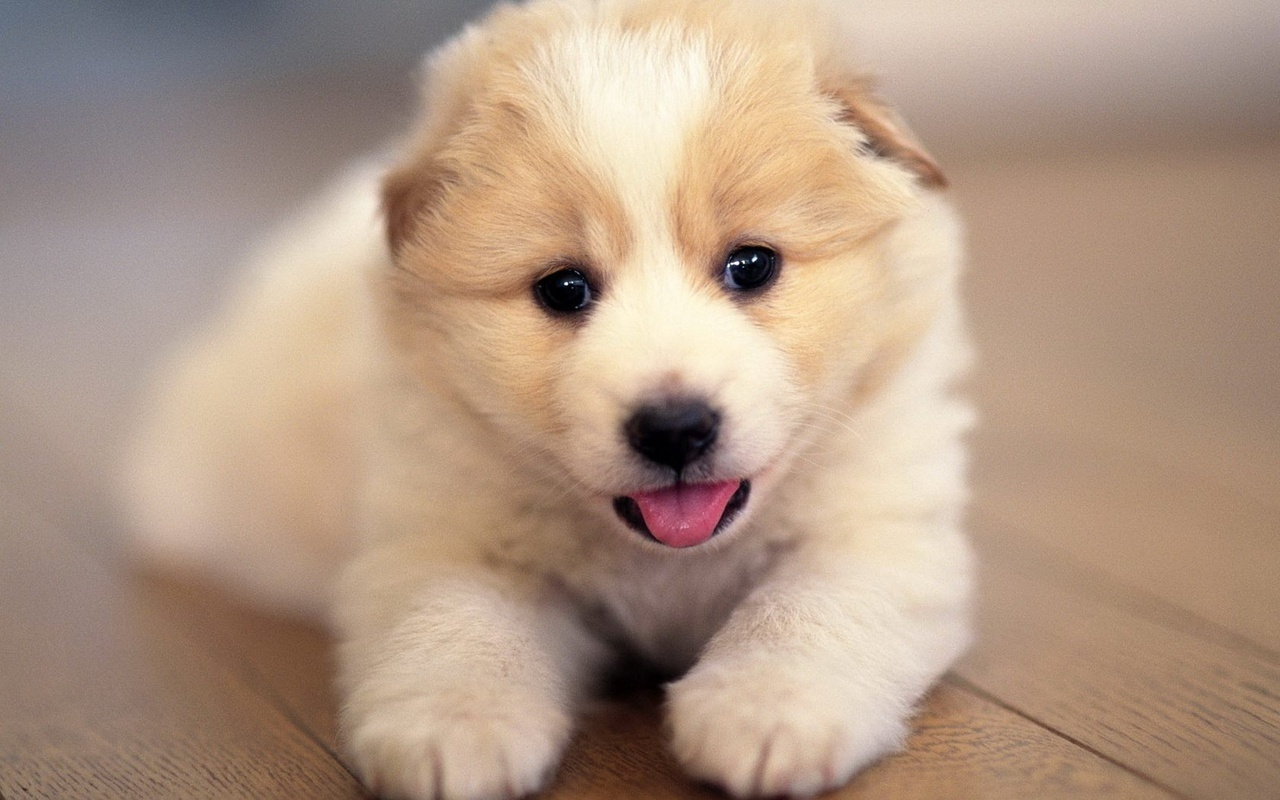
\includegraphics[width=3cm]{images/cutdog}}\\
		\vspace{.5cm}
		\uncover<2->{\includegraphics[width=2.5cm]{images/cutbaby}}
	    \hspace{1cm}
	    \uncover<3->{ \includegraphics[width=2cm]{images/pottery}}
	\end{center}
    \uncover<7>{$\rightarrow$ What mechanism drive the evolution of such traits?\\
    \invisible<1->{$\rightarrow$ What mechanism }generate such pattern?}
\end{frame}

\begin{frame}{What Generate Those Cultural changes?}
	Simple mechanisms (Bentley et al, 2004):
	\begin{itemize}
		\item<2->Random Copy 
		\item<3-> Frequency biased (conformist/anti-conformist\dots)
		\item<4->\dots	
	\end{itemize}
	\uncover<2>{\begin{figure}
		\begin{columns}
			\begin{column}{.8\textwidth}
				\centering
				\includegraphics[width=.6\textwidth]{images/powerlawrepartition.jpg}
			\end{column}
			\begin{column}{.3\textwidth}
				\tiny
				Square: male names\\
				Circle: female names\\
				Dotted and plain lines: model result with different copy probabilities.\\
			From Bentley et al,~2004.
			\end{column}
		\end{columns}
	    \end{figure}}
\end{frame}

\section{Economic Traits}


\begin{frame}
	\begin{center}
	    What if such mechanisms act on traits linked to economics?
	\end{center}
\end{frame}

\begin{frame}{A social trait and economic value}
	\begin{center}
	    \only<1>{\includegraphics[width=.8\textwidth]{images/boubou1.png}}
	    \only<2>{\includegraphics[width=.8\textwidth]{images/boubou2.png}}
	    \only<3>{\includegraphics[width=.8\textwidth]{images/boubou3.png}}
	\end{center}
\end{frame}

\begin{frame}{Co-evolution of Economy and Culture}

%How Simple Cultural Dynamics influence Economy That in turn will influence cultural dynamics.
    \vspace{2cm}
    \begin{center}
	\begin{overlayarea}{\textwidth}{\textheight}
	    \only<1>{\includegraphics[width=\textwidth]{images/map1.png}}
	    \only<2>{\includegraphics[width=\textwidth]{images/map2.png}}
	    \only<3>{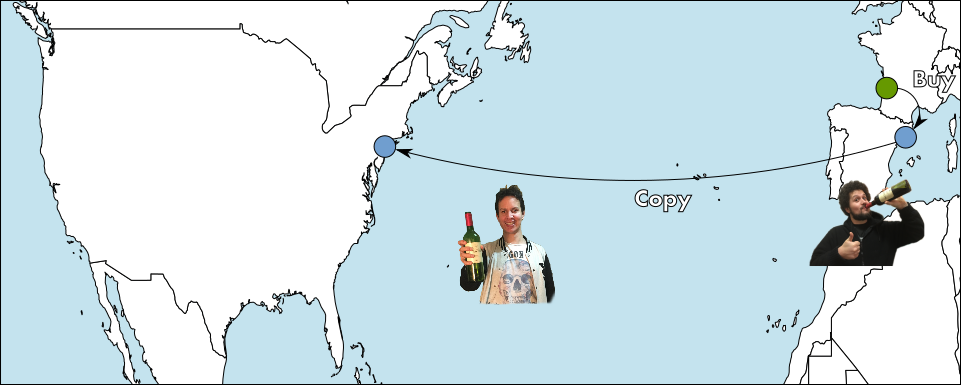
\includegraphics[width=\textwidth]{images/map3.png}}
	    \only<4>{\includegraphics[width=\textwidth]{images/map4.png}}
	    \only<5>{\includegraphics[width=\textwidth]{images/map5.png}}
	    \only<6>{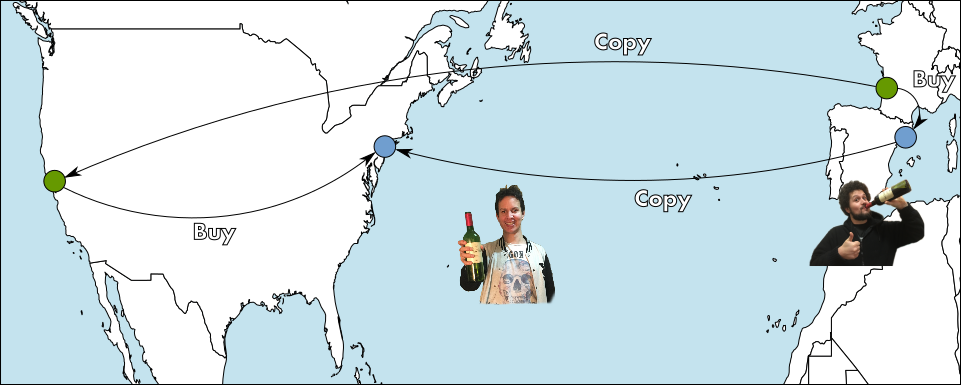
\includegraphics[width=\textwidth]{images/map6.png}}
	    \only<7>{\includegraphics[width=\textwidth]{images/map7.png}}
	    \only<8>{\includegraphics[width=\textwidth]{images/map8.png}}
	    \only<9>{\includegraphics[width=\textwidth]{images/map9.png}}
	    %\only<10>{\includegraphics[width=\textwidth]{images/map10.png}}
	    %\only<11>{\includegraphics[width=\textwidth]{images/graph1.png}}
	    %\only<12>{\includegraphics[width=\textwidth]{images/graph2.png}}
	    %\only<13>{\includegraphics[width=\textwidth]{images/graph3.png}}
	\end{overlayarea}

    \end{center}
\end{frame}



\section{ABM Framework}


\begin{frame}{General Framework}
    
    \begin{center}
	\includegraphics[width=.8\textwidth]{images/cooev.png}	
    \end{center}
\end{frame}
	
\begin{frame}{Agent Based Model}
    Inpsired by economists doing ACE (Agent-based Computation Economics):
    \begin{center}
	Gintis 2007, 2009, Gintis \& Mantel 2012, Chen et al. 2017\dots 
    \end{center}
    
    \begin{itemize}
	\item Simple decentralized economy
	\item Agent produce and exchanges goods
	\item Agents can socially learn form each other and ``innovate''
	\item Reach Walrasian ``general equilibrium''
    \end{itemize}
\end{frame}


\begin{frame}{Results: Economic Dynamics}
	\begin{figure}
	    \caption{Example for 3 goods and 500 agents}
	    \begin{columns}
		\column{.5\textwidth}
		\includegraphics[height=\textwidth]{images/ClearingPriceDistanceEvolutionForTrade-G3N500.pdf}\\
	    \end{columns}
		@~Equilibrium: personal values  $\rightarrow$ optimal (shared) values.
	\end{figure}
	
\end{frame}

\begin{frame}{Historical Case Study}
    \footnotesize
    \vspace{.5cm}
Change in distribution of Tableware in the East Roman Empire, -25BC 150AC:
    \begin{itemize}
	\item 5 types of wares 
	\item Distribution among 222 sites
	\item 5121 ware dataset
 \end{itemize}

 \begin{figure}
     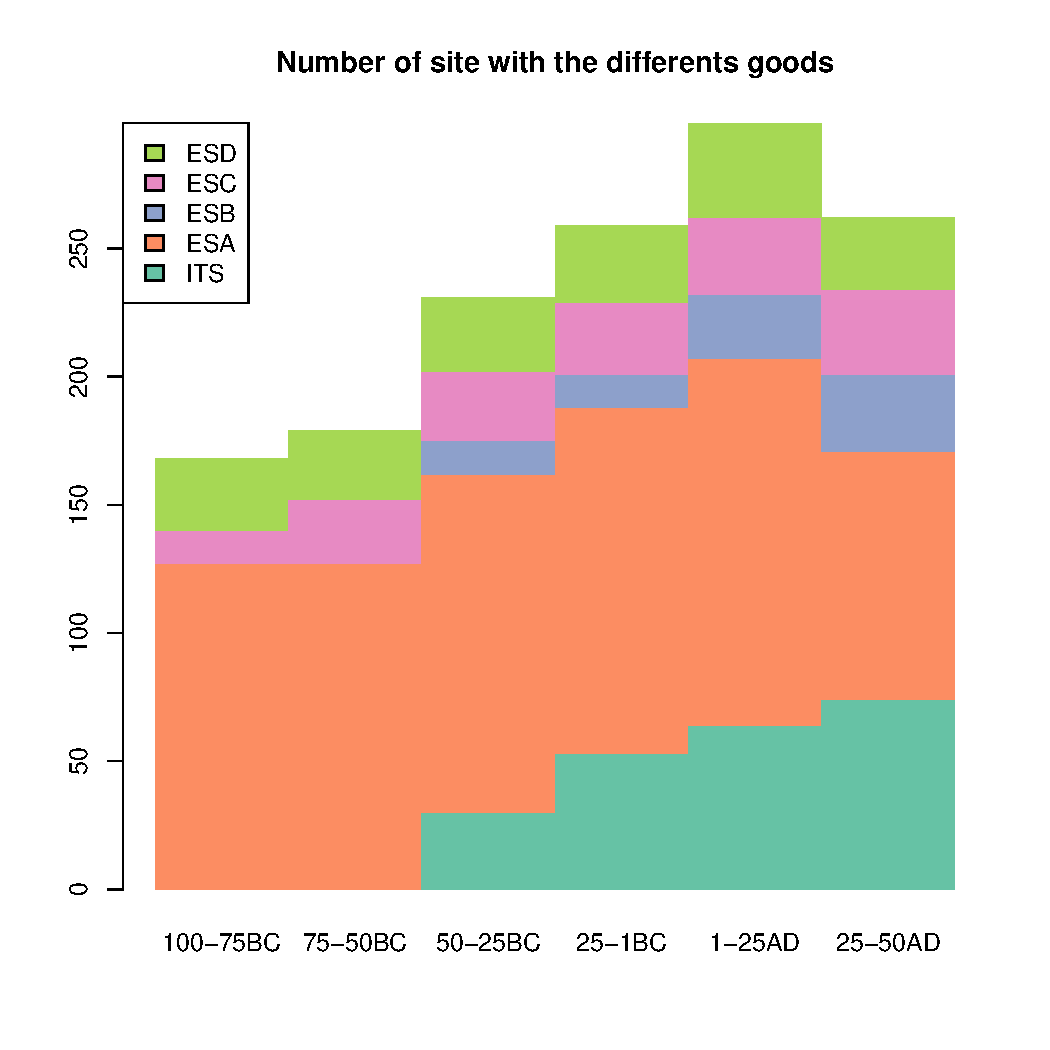
\includegraphics[width=.45\textwidth]{images/hmNbSiteWGoodData.pdf}
     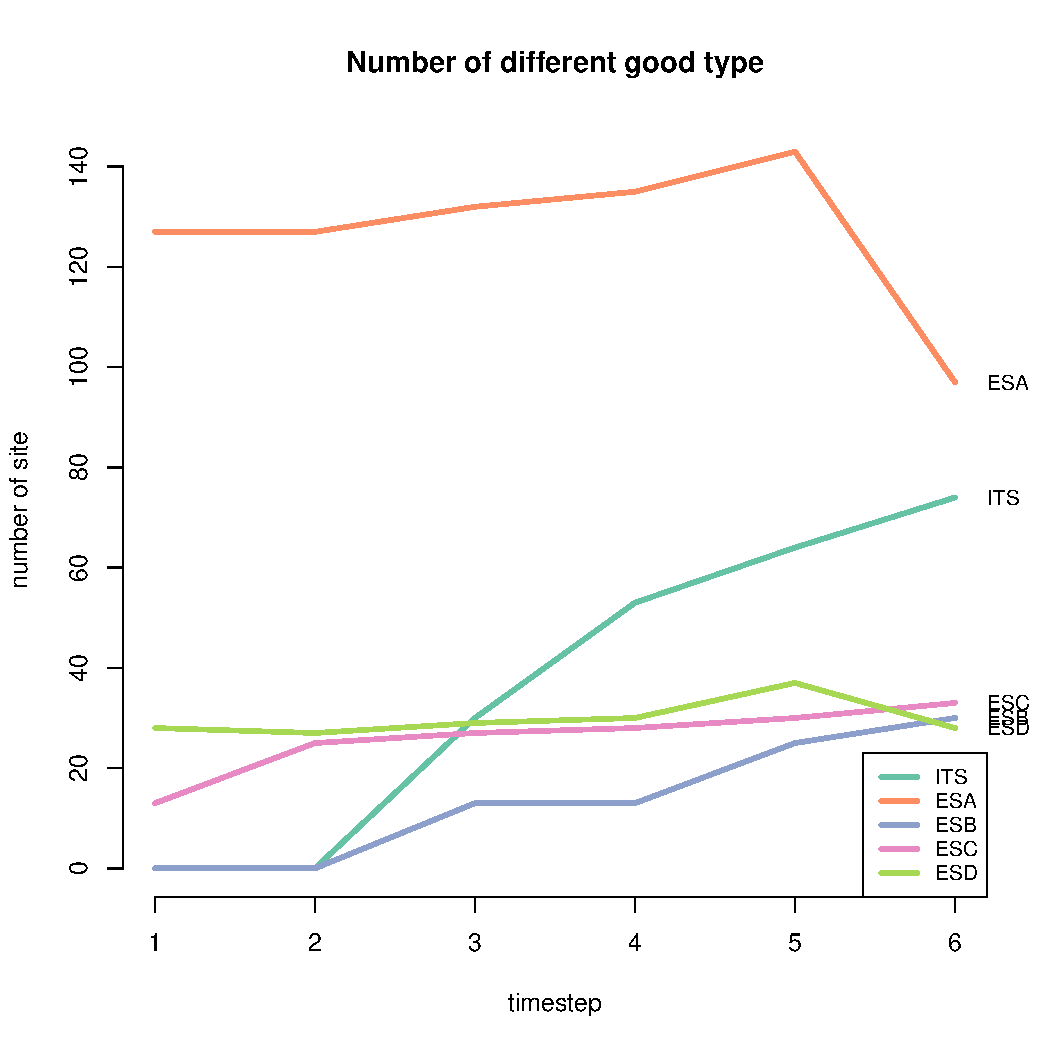
\includegraphics[width=.45\textwidth]{images/plotNbSiteWGoodData.pdf}
     
 \end{figure}
 \begin{center}
     \tiny other info: Site with different number of good
 \end{center}
\end{frame}

\begin{frame}{Specification of the model}
    Calibrate the simulation:
    \begin{itemize}
	\item 1000 agents
	\item 5 goods (+money) to appear 
	\item 200 ``cultural'' steps 
	\item 3000 ``trade'' steps ($15\times200$)
	\item every 40 cultural steps (ie $600$ trade step) a new good appears.
	\item $\approx 35min$
    \end{itemize}
\end{frame}

\begin{frame}{Experimental framework}
Individual  vs Social learning  ( $\mu$ vs $\lambda$ )
    \begin{itemize}
	\item Test change in $\mu$ the innovation rate (``I randomly change a price'')\\
	    \hspace{.2cm} $\mu \in \{0.001,0.01,0.1,1\}$
	\item Test change in $\lambda$, factor to increase the proba. to copy someone better than me\\
	    \hspace{.2cm} $\lambda \in \{0.0001,0.001,0.01,0.1,1,10\}$
	\item ( also $\mu$ amplitude, \emph{ie} amplitude of price change when I decide to do so, not shown here)
	\item  $ 6 \times 4 = 24$ setup, 50s simulation each
    \end{itemize}
\end{frame}


\begin{frame}{Number of site with good 'N'}
    \small
Data \hfill Exp1 \hfill Exp2 \hfill Expe3 
	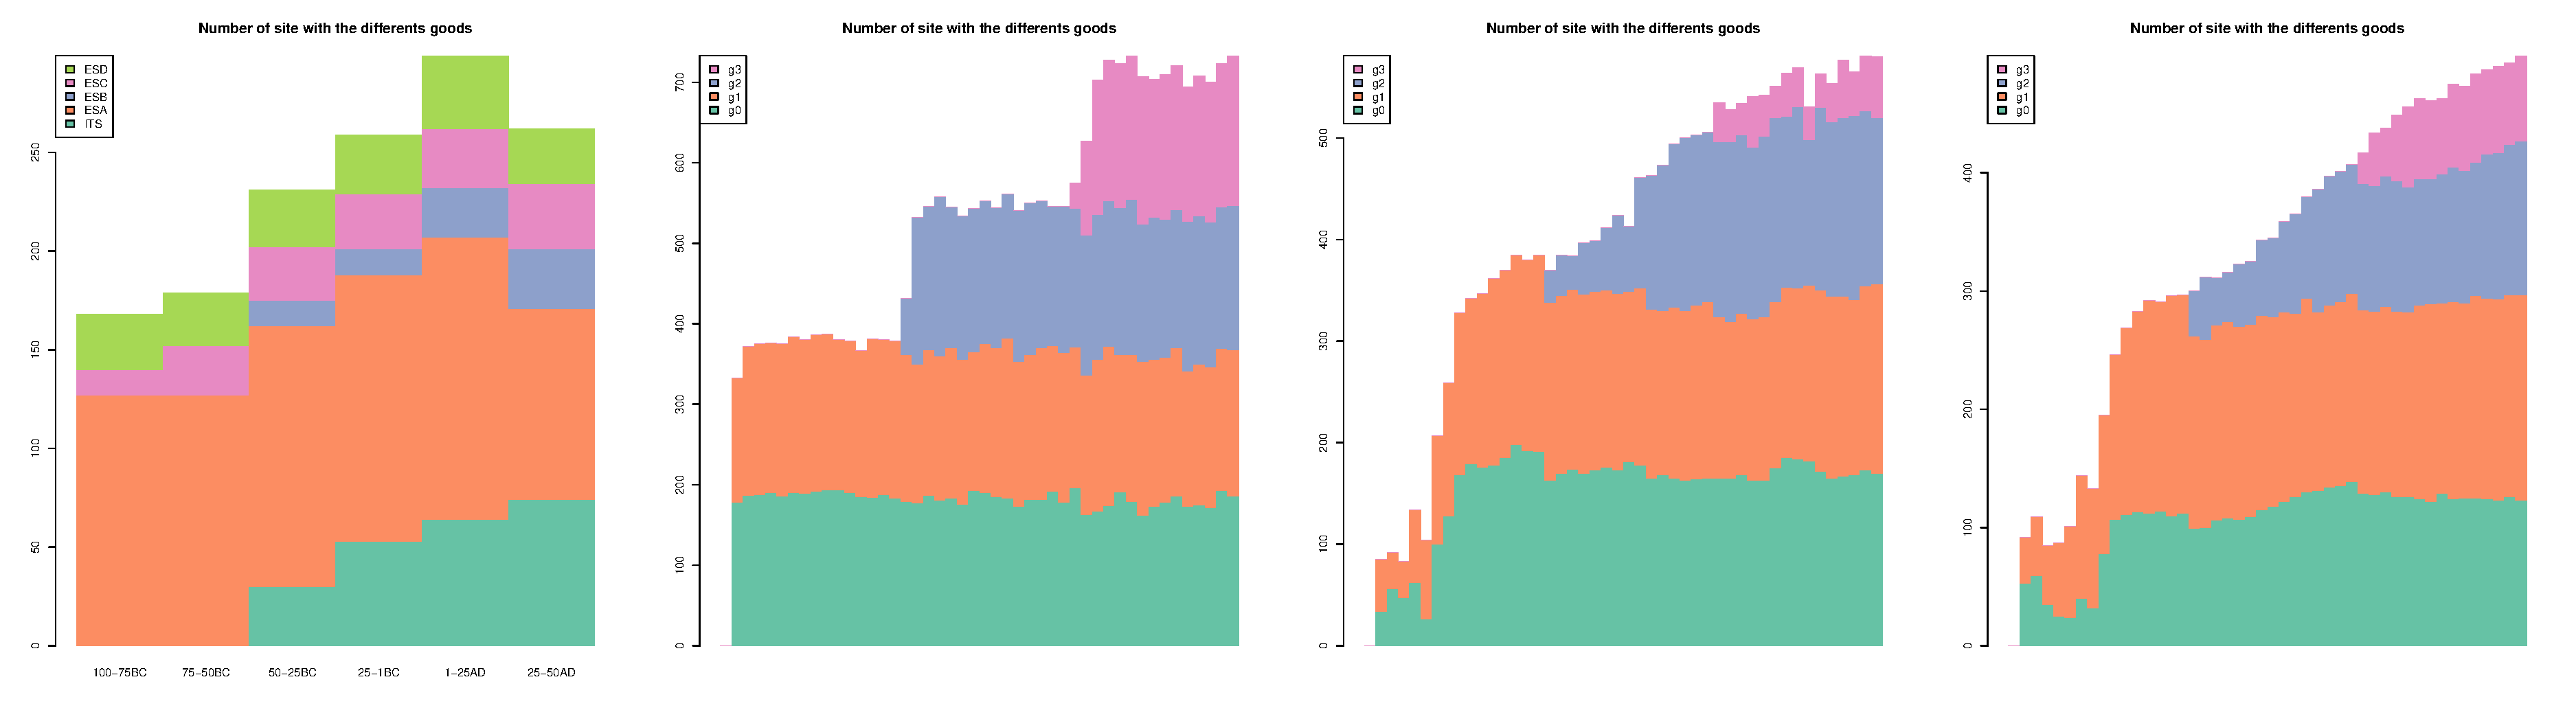
\includegraphics[width=\textwidth]{images/hmNbSiteWGoodN.pdf}\\
	\includegraphics[width=\textwidth]{images/plotNbSiteWGoodN.pdf}\\
\end{frame}

\begin{frame}{Number of site with 'N' different goods}
    \centering
    \tiny
 Exp1 \hfill Exp2 \hfill Expe3 
	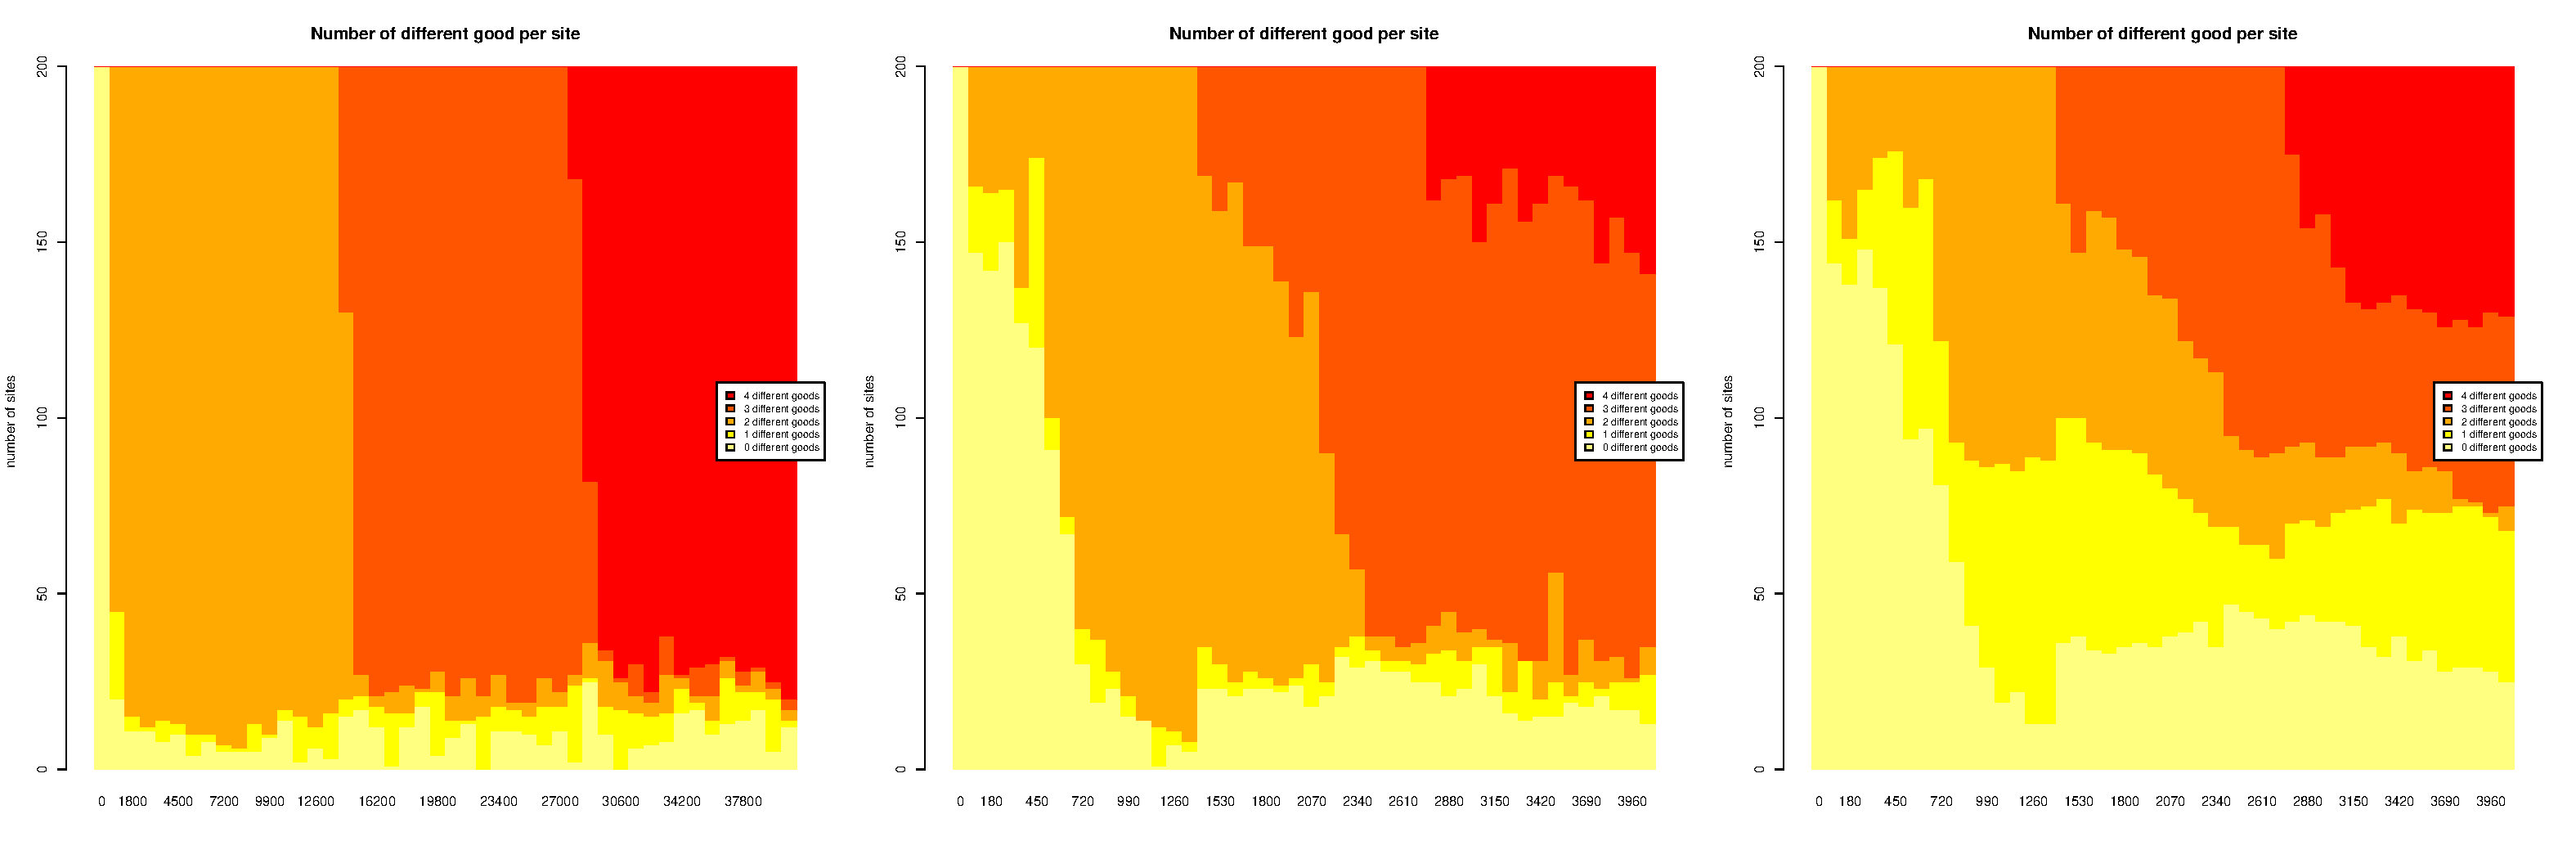
\includegraphics[width=.95\textwidth]{images/hmNbGoodPerSite.pdf}\\
	\vfil
	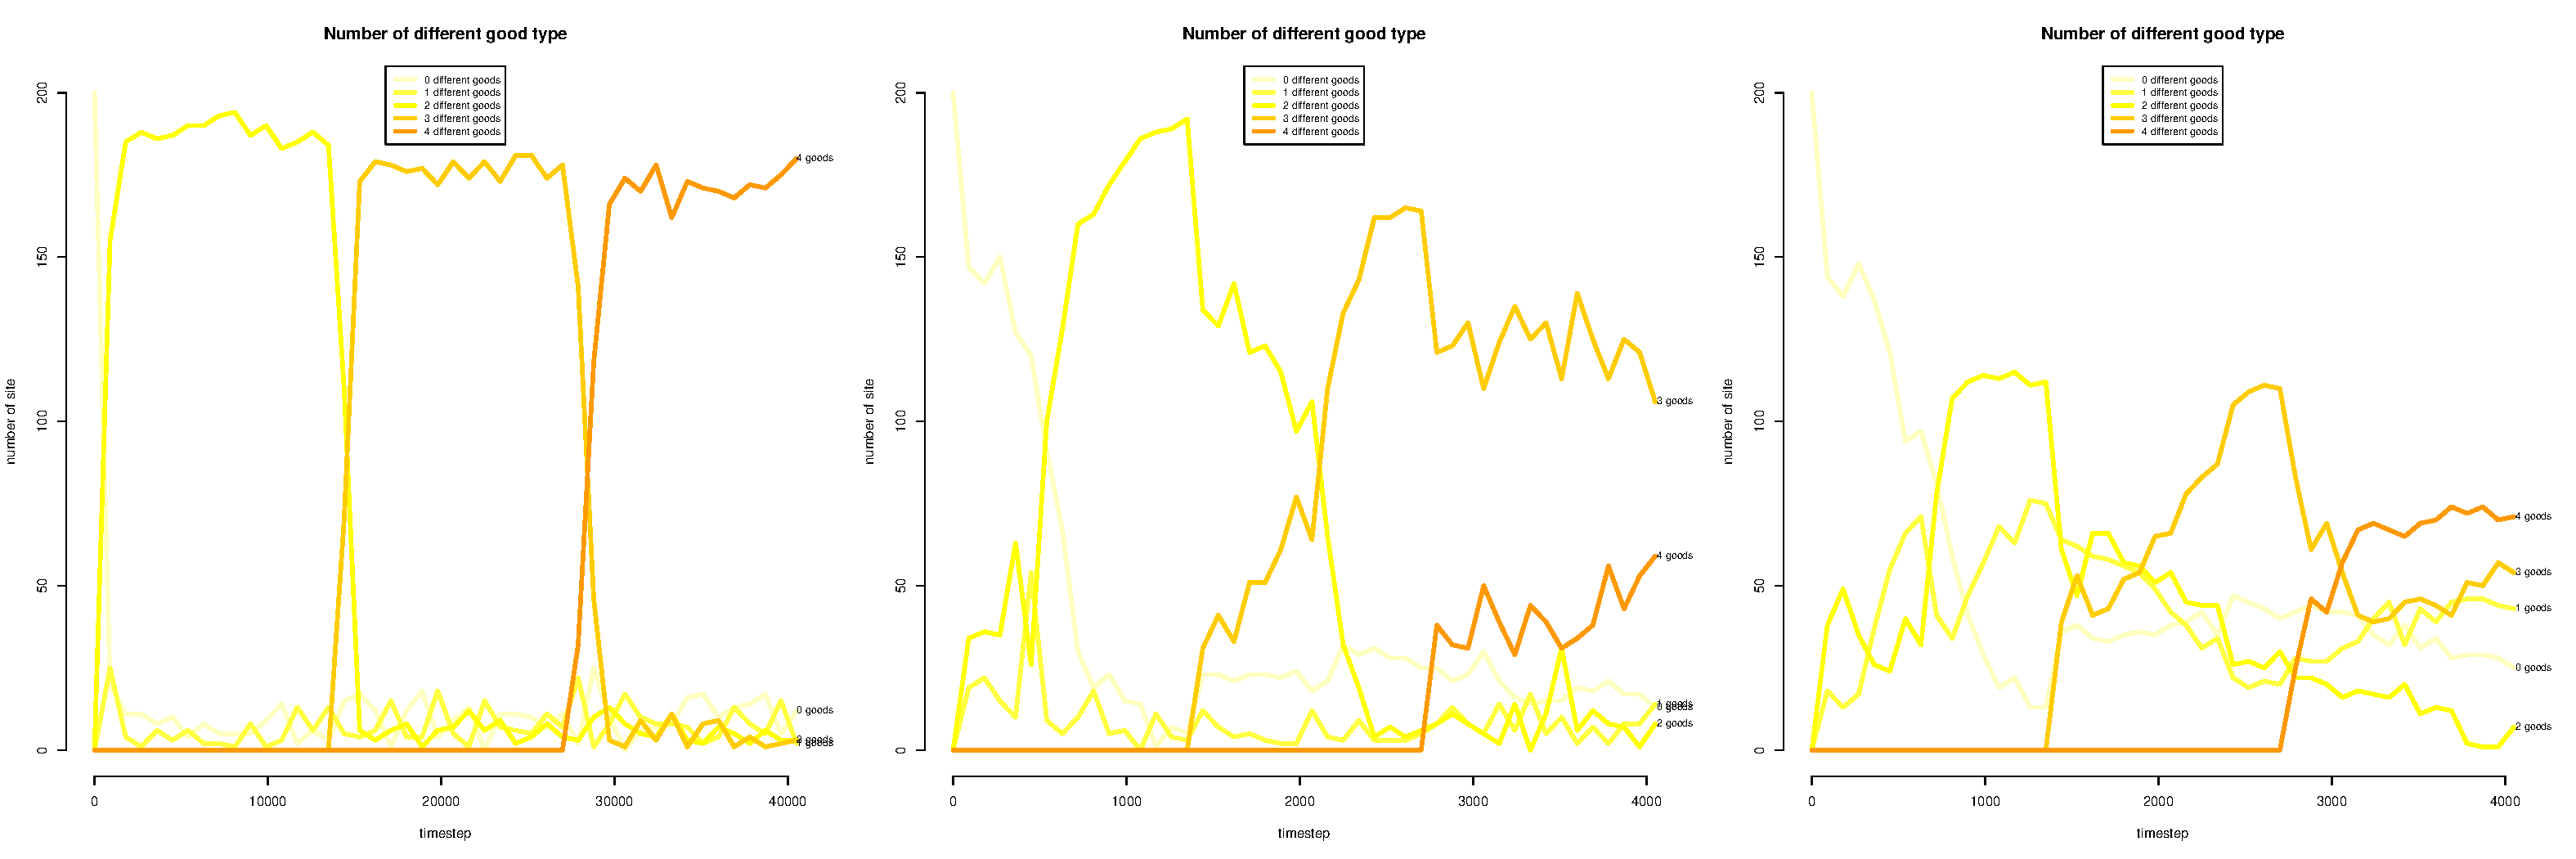
\includegraphics[width=.95\textwidth]{images/plotNbGoodPerSite.pdf}\\
\end{frame}


\end{document}


